\documentclass[tikz]{standalone}\input{pre.tex}\begin{document}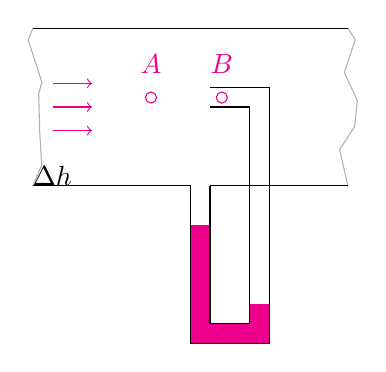
\begin{tikzpicture}

	\fill[magenta] (2,0)++(0,-0.5) rectangle ++ (0.25,-1.5);
	\fill[magenta] (2.75,0)++(0,-1.5) rectangle ++ (0.25,-0.5);
	\fill[magenta] (2,0)++(0,-2) rectangle ++ (1,0.25);

	\draw[black!30, decoration={random steps, amplitude=1.5mm}, decorate] (0,0) -- ++(0,2);
	\draw[black!30, decoration={random steps, amplitude=1.5mm}, decorate] (4,0) -- ++(0,2);
	\draw (0,2) -- ++(4,0); 
	\draw (0,0) -- ++(2,0) -- 
						++ 	(0,-2) 	--
						++ 	(1,0) 	--
						++ 	(0,2) 	--
						++	(1,0); 
	\draw (2.25,0) -- ++ (0,-1.75) -- ++ (0.5,0) -- ++ (0,2.75) -- ++(-0.5,0) coordinate (c);

	\draw (c) ++ (0,0.25) -- ++ (0.75,0) -- ++(0,-1.25);
	\draw (2.25,0) -- ++ (1,0);

	\draw[magenta] (1.5,1.12) circle (2pt) node[above, yshift=0.5em] {$A$};
	\draw[magenta] (2.4,1.12) circle (2pt) node[above, yshift=0.5em] {$B$};

	\draw[magenta,->] (0.25,1) -- ++(0.5,0);
	\draw[magenta,->] (0.25,0.7) -- ++(0.5,0);
	\draw[magenta,->] (0.25,1.3) -- ++(0.5,0);
	% Draw line annotation
	% Input:
	%   #1 Line offset (optional)
	%   #2 Line angle
	%   #3 Line length
	%   #5 Line label
	\begin{scope}[xshift=3cm, yshift=-1.5cm]
	  \lineann[2]{90}{1}{$\Delta h$}
	\end{scope}

\end{tikzpicture}\end{document}